% Chapter - Player Study - Physical Health effects
\chapter{Physical Health Effects}
\label{chapter:player-study-physical}
\lhead{Chapter \ref{chapter:player-study-physical}. \emph{Player Study - Physical Health Effects}}

This chapter examines the survey results in the context of determining th game's effect on the physical health of its players. The questions in Table \ref{tbl:rg2-survey-questions} and their answers are the main focus of this chapter, but relevant answers to other questions are also included.

\section{Results for Change in Physical Activity}

This section presents the results for the player survey questions related to Research Questions \ref{RQ2.1}, \ref{RQ2.2} and \ref{RQ2.3}. A total of 2193 subjects responded to the questions \emph{"In an average week, how much time did you spend on physical activities (e.g. walking, running or biking) before you started playing Pokémon Go?"} and \emph{"In an average week, how much time do you spend on physical activities since you started playing Pokémon Go?"}. Table \ref{tbl:physical-activity-before-and-after} shows the number of responses to each question (column 2 and 3 respectively), as well as the change \todo{(should it say delta?)}, within each time category. Percentages for the \emph{Before} and \emph{After} columns are the percentage of total respondents for the respective category, while the percentage in the \emph{Change} column shows the relative increase or decrease (negative percentages) for that category. Note that the percentages are rounded to the closest integer, and due to rounding errors, the percentages in column 2 and 3 sum to 101 \% and 99 \% respectively.

\begin{table}[h]
	\centering
	\caption{Physical activity before and after Pokémon GO}
	\label{tbl:physical-activity-before-and-after}
	\begin{tabular}{|l|c|c|c|}
		\hline
		\textbf{Hours of activity} & \textbf{Before} & \textbf{After} & \textbf{Change} \\\hline\hline
		30 minutes or less	& 395 & 32 & -363\\
							& 18\% & 1\% & -92\%\\\hline
		An hour or less & 324 & 107 & -217\\
						& 15\% & 5\% & -67\%\\\hline
		2 hours or less & 384 & 268 & -116\\
						& 18\% & 12\% & -30\%\\\hline
		4 hours or less & 477 & 515 & 38\\
						& 22\% & 23\% & 8\%\\\hline
		8 hours or less & 394 & 566 & 172\\
						& 18\% & 26\% & 44\%\\\hline
		12 hours or less	& 132 & 365 & 233\\
							& 6\% & 17\% & 177\%\\\hline
		20 hours or less	& 61 & 206 & 145\\
							& 3\% & 9\% & 238\%\\\hline
		More than 20 hours	& 26 & 134 & 108\\
							& 1\% & 6\% & 415\%\\\hline
	\end{tabular}
\end{table}

Where Table \ref{tbl:physical-activity-before-and-after} showed the number of respondents in each time range before and after Pokémon GO, Table \ref{tbl:physical-activity-changed-category} shows the number and portion of respondents who remained in their category, went up one or more categories, or down one or more categories. This is a good indicator of how many respondents became more or less physically active, but will not be exact as some players became more active within the same range while others became less active within the same range. \todo{Should this paragraph and table be in analysis?}

\begin{table}[h]
	\centering
	\caption{How many respondents changed physical activity categories?}
	\label{tbl:physical-activity-changed-category}
	\begin{tabular}{|l|c|c|c|}
		\hline
		\textbf{Initial category} & \textbf{Increased} & \textbf{Stable} & \textbf{Decreased}\\
		\hline\hline
		30 minutes or less	& 372	& 23	& n/a\\
		& 94\%	& 6\%	& \\\hline
		An hour or less		& 276	& 44	& 4\\
		& 85\%	& 14\%	& 1\%\\\hline
		2 hours or less		& 321	& 44	& 6\\
		& 84\%	& 15\%	& 1\%\\\hline
		4 hours or less		& 332	& 136	& 9\\
		& 70\%	& 28\%	& 2\%\\\hline
		8 hours or less		& 220	& 166	& 8\\
		& 56\%	& 42\%	& 2\%\\\hline
		12 hours or less	& 59	& 65	& 8\\
		& 45\%	& 49\%	& 6\%\\\hline
		20 hours or less	& 25	& 32	& 4\\
		& 41\%	& 52\%	& 7\%\\\hline
		More than 20 hours	& n/a		& 23	& 3\\
		&	& 88\%	& 12\%\\\hline
		\hline
		Total				& 1605	& 546	& 42\\
		& 73\%	& 25\%	& 2\%\\\hline
	\end{tabular}
\end{table}

Figure \ref{fig:change-in-physical-activity} shows the change in physical activity relative to previous activity. The X-axis show weekly physical activity before Pokémon GO, while the Y-axis shows weekly physical activity after they started playing Pokémon GO, with both axes ranging from \emph{Less than 30 minutes} to \emph{More than 20 hours}. The green cells are players who increased their physical activity, while red cells are players who became less physically active after they started playing. Darker shades signify a larger difference, while the white cells indicate no change. \todo{Should this paragraph and figure be in analysis?}

\begin{figure}[h]
	\centering
	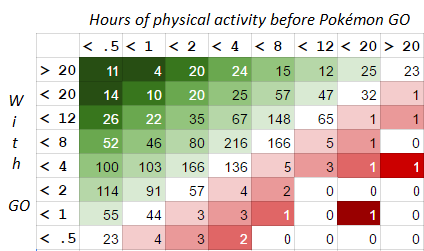
\includegraphics{Figures/change-in-physical-activity-table-colors}
	\caption{Change in physical activity with Pokémon GO}
	\label{fig:change-in-physical-activity}
\end{figure}

Respondents were also asked what activities lead to the increase in their physical activity, if they had become more physically active. Table \ref{tbl:physical-activity-sources} shows the number of respondents for each option out of 1823 respondents who reported an increase in physical activity.

\begin{table}[h]
	\centering
	\caption{Reasons for increased physical activity from Pokémon GO}
	\label{tbl:physical-activity-sources}
	\begin{tabular}{|c|c|c|c|}
		\hline
		\textbf{Detours} & \textbf{Errands} & \textbf{Pokéhunting} & \textbf{Other}\\\hline\hline
		1136 & 636 & 1576 & 89\\
		62\% & 35\% & 86\% & 5\%\\\hline
	\end{tabular}
\end{table}

It should be noted that 31 of these respondents (less than 2 \%) also chose the \emph{Not applicable} option, but it is uncertain what the implication of this is, given that they also selected other options. 25 of these 31 chose the same category for activity before and after, but because they are ranges it is still possible that they have increased activity within that range. The 6 remaining of those 31 reported more physical activity after Pokémon GO than before, so we can safely ignore the \emph{Not applicable} choice in their case. \todo{Should this be in Section \ref{sec:problems-with-survey} instead?}

The three categories \emph{Detours}, \emph{Errands} and \emph{Pokéhunting} were further explained in the question's options, see Appendix \ref{appendix:survey} \todo{(so I assume I don't have to repeat them here? Or should I?)}. Common examples of other activities leading to an increase in physical activity were players with dogs who walked them longer and more frequently to get in more play time or distance for their eggs, players who would walk during their breaks at work instead of sitting down, and players who went for longer or more frequent runs than previously. Many players who knew they should be going for walks but previously wouldn't have, used Pokémon GO as a motivation to get outside and move around. Others found they enjoyed moving more and were motivated to start more rigorous exercise, while some even learned how to ride a bicycle so they could play more efficiently. \todo{Should I mention the respondents who said they increased physical activity for reasons unrelated to Pokémon GO? If so, here or in Section \ref{sec:problems-with-survey}?}

\section{Analysis of Results for Change in Physical Activity}

The results were overwhelmingly positive. As seen in Table \ref{tbl:physical-activity-changed-category}, 73 \%, nearly three out of every four respondents, increased their physical activity enough to move up at least one category in physical activity after Pokémon GO compared to before. Table \ref{tbl:physical-activity-increased-multiple-categories} shows how many respondents from each initial category moved 2, 3, 4, 5 or 6 categories. Table \ref{tbl:physical-activity-average-categories-increased} shows how many categories players on average increased depending on their initial category. The \emph{Only increased} category shows the average increase for those who did in fact increase physical activity, while \emph{All} shows the numbers for all respondents who started within the respective category, including those who remained stable and those who decreased physical activity. \todo{Should these tables be moved to results?}

\begin{table}[h]
	\centering
	\caption{How many respondents increased physical activity by multiple categories?}
	\label{tbl:physical-activity-increased-multiple-categories}
	\begin{tabular}{|l|c|c|c|c|c|}
		\hline
		\textbf{Initial category} & \textbf{\( \geq2 \)} & \textbf{\( \geq3 \)} & \textbf{\( \geq4 \)}	& \textbf{\( \geq5 \)} & \textbf{\( \geq6 \)}\\
		\hline\hline
		30 minutes or less	& 317	& 203	& 103	& 51	& 25\\
							& 80\%	& 51\%	& 26\%	& 13\%	& 6\%\\\hline
		An hour or less		& 185	& 82	& 36	& 14	& 4\\
							& 57\%	& 25\%	& 11\%	& 4\%	& 1\%\\\hline
		2 hours or less		& 155	& 75	& 40	& 20	& n/a\\
							& 40\%	& 20\%	& 10\%	& 5\%	&\\\hline
		4 hours or less		& 116	& 49	& 24	& n/a	& n/a\\
							& 24\%	& 10\%	& 5\%	&		&\\\hline
		8 hours or less		& 72	& 15	& n/a	& n/a	& n/a\\
							& 18\%	& 4\%	& 		&		&\\\hline
		12 hours or less	& 12	& n/a	& n/a	& n/a	& n/a\\
							& 9\%	& 		&		&		&\\\hline
		\hline
		Total				& 857	& 424	& 203	& 85	& 29\\
							& 39\%	& 19\%	& 9\%	& 4\%	& 1\%\\\hline
	\end{tabular}
\end{table}

\begin{table}[h]
	\centering
	\caption{How many categories on average did players increase physical activity?}
	\label{tbl:physical-activity-average-categories-increased}
	\begin{tabular}{|l|c|c|}
		\hline
		\textbf{Initial category} & \textbf{Only increased} & \textbf{All}\\
		\hline\hline
		30 minutes or less	& 2.91	& 2.74\\
		An hour or less		& 2.16	& 1.83\\
		2 hours or less		& 1.90	& 1.57\\
		4 hours or less		& 1.57	& 1.06\\
		8 hours or less		& 1.40	& 0.75\\
		12 hours or less	& 1.20	& 0.45\\
		20 hours or less	& 1.00	& 0.23\\
		More than 20 hours	& n/a	& -0.27\\
		\hline
		Total				& 2.00	& 1.43\\\hline
	\end{tabular}
\end{table}

Because more than 92 \% of our respondents are adults by the WHO's definition of adults being aged 18-16, we are going to focus on the recommendations for adults. As discussed in Section \ref{sec:lit-study-physical-activity}, the WHO recommends that adults do at least 150 minutes of moderate-intensity physical activity per week. Using this recommendation, we categorize the players who are physically active less than this (the lower three categories) as \emph{Low activity} players. Respondents within the \emph{4 hours or less} and \emph{8 hours or less} categories will be categorized as \emph{Moderate activity} players, while the three remaining categories are \emph{High activity} players.

\begin{table}
	\centering
	\caption{Low/moderate/high activity players}
	\label{tbl:physical-activity-low-moderate-high}
	\begin{tabular}{|l|c|c|c|c|}
		\hline
		\textbf{Activity level}	& \textbf{Before}	& \textbf{After}	& \textbf{Change}	& \textbf{Categories increased}\\
		\hline\hline
		Low		& 1103	& 407	& -696	& 2.06\\
				& 50\%	& 19\%	& -63\%	&\\\hline
		Moderate& 871	& 1081	& 210	& 0.92\\
				& 40\%	& 49\%	& 24\%	&\\\hline
		High	& 219	& 705	& 486	& 0.31\\
				& 10\%	& 32\%	& 222\%	&\\\hline
	\end{tabular}
\end{table}

We see that while 50 \% of respondents were of low activity before Pokémon GO, this group only consisted of 19 \% of the respondents after Pokémon GO, a decrease of over 60 \%. The effect was larger for the lower activity ranges, where the number of respondents who had previously been active 30 minutes or less per week decreased by 92 \%, while the number who had previously been active between 1 and 2 hours per week only decreased by 30 \%. This is partly because the \emph{2 hours or less} category also saw an influx of players from the lower categories, but also because the lower ranges were narrower and thus easier to transcend. However, from Table \ref{tbl:physical-activity-average-categories-increased} we see that more than 50 \% of the respondents from the \emph{30 minutes or less} category increased their activity to a moderate level by jumping 3 or more categories, with the average number of categories increased for respondents initially placed in this category was 2.74.

The number of moderate activity players increased by 24 \%, which does not seem like a huge increase. However, paired with the fact that the number of high activity players more than tripled with a 222 \% increase, the number becomes more impressive, as this means the moderate activity category also "lost" quite a few of the players originally in this category. Respondents in the moderate activity category increased activity by a little less than one category on average. While this is not an enormous shift for these players, it places them safely within the range of the WHO's recommended weekly activity.

High activity players increased activity by 0.31 categories on average, with the majority of these increases coming from the players who had initially been active 12 hours or less. The initial members of the \emph{More than 20 hours} category decreased by 0.27 categories on average. The sample size was very small, however, consisting of only 26 respondents initially. The 0.27 category decrease is the result of three individuals and does not take into account that those in the \emph{More than 20 hours} category were unable to increase in category and that there were some respondents who mentioned in comments that they had in fact increased activity by 5-10 hours. It is however plausible that balancing a high physical activity week with playing Pokémon GO can be difficult, resulting in a slight decrease in physical activity from participating in game activities such as "camping" lures or nests. \todo{More on low-movement activities such as "camping".}

\todo{Althoff et al. ("Influence of Pokémon Go on Physical Activity ...") is highly relevant here and probably has some}

\todo{Type of activity shows that it's likely things regress after playing stops, which is in line with follow-up surveys. Some people were motivated to start exercise, though!}

\todo{Only 19 \% left in low activity!}

%\section{Benefits}

%\todo{Increased physical activity, weight loss and general feeling of wellness, skipping unhealthy activities}

%\section{Neglect and Negative Behavior}


% Chapter
\chapter{Mental Health Effects}
\label{chapter:player-study-mental}
\lhead{Chapter \ref{chapter:player-study-mental}. \emph{Player Study - Mental Health Effects}}

\todo{Maybe combine the following into just two sections - negative and positive}

\section{Social Interaction}
\label{sub:mental-health-social}

\todo{Mention division of tasks (searching for nearby pokes, scoping out gyms, and transporter/player), and that players on different teams still can cooperate and be on good terms}

\section{Exercise}

\section{A Sense of Purpose}

\section{Disappointment}

\section{Negative Behavior and Adversarial Relationships}